\documentclass[12pt,a4paper]{article}

\usepackage{graphicx,framed,enumerate,multicol}
\usepackage{amsmath,latexsym,amsfonts,mathtools,array}
\usepackage{tikz}
\usepackage{tkz-graph}
%\usepackage[margin=0.45in]{geometry}


%\usepackage{fullpage}

\begin{document}

\begin{center}
\textsc{\Huge \textbf{Train Game Diary}}
\end{center}

\section*{Brute force vs Graph approach}
\noindent \texttt{29/12/15}\\
\subsection*{Brute Force}
\noindent Currently the program uses a brute force approach to find possible solutions. Consider the digits $\lbrace1,2,3,4\rbrace$ and the set of operations $\lbrace+,-,\times,\div\rbrace$. First, all possible permutations of the operations are generated.
\begin{framed}
\begin{multicols*}{5}
\noindent 
$$+ + +$$
$$+ + -$$
$$+ + \times$$
$$+ + \div$$
$$+ - -$$
$$+ - \times$$
$$+ - \div$$
$$+ \times \times$$
$$+ \times \div$$
$$+ \div \div$$
$$- - -$$
$$- - \times$$
$$- - \div$$
$$- \times \times$$
$$- \times \div$$
$$- \div \div$$
$$\times \times \times$$
$$\times \times \div$$
$$\times \div \div$$
$$\div \div \div$$
\end{multicols*}
\end{framed}

Next, all the possible permutations of the digits are generated.
\begin{framed}
\begin{multicols}{4}
\noindent 
$$1 2 3 4$$
$$1 2 4 3$$
$$1 3 2 4$$
$$1 3 4 2$$
$$1 4 2 3$$
$$1 4 3 2$$
$$2 1 3 4$$
$$2 1 4 3$$
$$2 3 1 4$$
$$2 3 4 1$$
$$2 4 1 3$$
$$2 4 3 1$$
$$3 1 2 4$$
$$3 1 4 2$$
$$3 2 1 4$$
$$3 2 4 1$$
$$3 4 1 2$$
$$3 4 2 1$$
$$4 1 2 3$$
$$4 1 3 2$$
$$4 2 1 3$$
$$4 2 3 1$$
$$4 3 1 2$$
$$4 3 2 1$$
\end{multicols}
\end{framed}

For each combination of operations, each digit set is applied.\\

For example, for the operation $+ + +$ the digits $1234$, $1243$, ... $4321$ are applied.
\begin{framed}
\noindent 
$$1+2+3+4$$
$$1+2+4+3$$
$$1+3+2+4$$
$$...$$
$$4+2+3+1$$
$$4+3+1+2$$
$$4+3+2+1$$
\end{framed}

Similarly, for the operation $+ + -$ the numbers $1234$, $1243$, ... $4321$ are applied.

\begin{framed}
\noindent 
$$1+2+3-4$$
$$1+2+4-3$$
$$1+3+2-4$$
$$...$$
$$4+2+3-1$$
$$4+3+1-2$$
$$4+3+2-1$$
\end{framed}

So on and so forth.\\

We use \texttt{eval} to evaluate each of these statements and let a solution be any combination of the digits and operations that equals $10$.\\

In our example there are 32 solutions.

\begin{framed}
$$1+2+3+4 = 10$$
$$1+2+4+3 = 10$$
$$...$$
$$4+2*3/1 = 10$$
$$4+3*2/1 = 10$$
\end{framed}

\subsection*{Brute Force Calculations}

\subsubsection*{Definitions}
Let set of digits to use $D = \lbrace d_1,~d_2,~d_3,~d_4~.~.~.~d_m \rbrace$\\
Let set of operations to use $O = \lbrace o_1,~o_2,~o_3,~o_4~.~.~.~o_n \rbrace$ where $m,n \in \mathbb{Z}$\\

\noindent $|D| = m = $ number of digits to use.\\
$|O| = n = $ number of operations you have at your disposal.

\subsubsection*{Valid statement}
\noindent A valid statement that can be evaluated is $$d_{p_{1}}~~o_{q_{1}}~~d_{p_{2}}~~o_{q_{2}}~~d_{p_{3}}~~o_{q_{3}}~~d_{p_{4}}~.~.~.~o_{q_{n}}~~d_{p_{m}}$$ where $p,q \in \mathbb{Z}$ such that $1 \leq p \leq m$ and $1 \leq q \leq n$.\\

\subsubsection*{Generating Permutations of Numbers}
\noindent $|D| = m$ (from above).\\

%\noindent Use $k$ numbers to form a valid statement.\\

\noindent Out of $m$ numbers, we are using all $m$ digits to generate a valid statement.\\

\noindent $m$ numbers to use, permute $m$ times, $^{m}\!P_{m}$.\\

$$^{m}\!P_{m} = \dfrac{m!}{(m-m)!} = \dfrac{m!}{(0)!} = \dfrac{m!}{1}  = m!$$

\subsubsection*{Generating Combinations of Operations (with Repetition)}
\noindent $|O|  = n$ (from above).\\
 
%\noindent Use $(m-1)$ operations to form a valid statement.

\noindent Out of $n$ operations, we are choosing $(n - 1)$ operations to generate a valid statement.\\

\noindent $n$ operations choose $n-1$ (with repetition), ${n + (n-1) -1 \choose (n-1)} $.\\

$$\dfrac{(n + (n-1) - 1)!}{(n-1)!(n-1)!} = \dfrac{(2n-2)!}{(n-1)!^2}$$ \\

\subsubsection*{Putting it together}

As mentioned earlier, 

\begin{framed}
\textit{For each combination of operations, each digit set is applied.}
\end{framed}

\noindent Therefore, in a brute force approach, we generate a total of 
\begin{framed}
$$\dfrac{(2n-2)!}{(n-1)!^2} \times m!$$ 
\end{framed}
statements to be evaluated.

\subsubsection*{An Application - Our Example}
Let set of digits to use $D = \lbrace 1, 2, 3, 4 \rbrace$\\
Let set of operations to use $O = \lbrace +, - , \times, \div \rbrace$\\

\noindent $|D| = m = 4$ digits to use\\
$|O| = n = 4$ operations at disposal\\

\noindent Number of brute force statements to evaluate $$\dfrac{(2n-2)!}{(n-1)!^2} \times m! = \dfrac{(2(4)-2)!}{((4)-1)!^2} \cdot (4)! = \dfrac{6!}{(3)!^2} \cdot 4! = 480$$

\subsubsection*{Complexity}

Algorithm time complexity $O(a^2)$. 

\pagebreak

\subsection*{Graph}

Instead, we can approach the problem from a tree-based problem.\\

\begin{center}

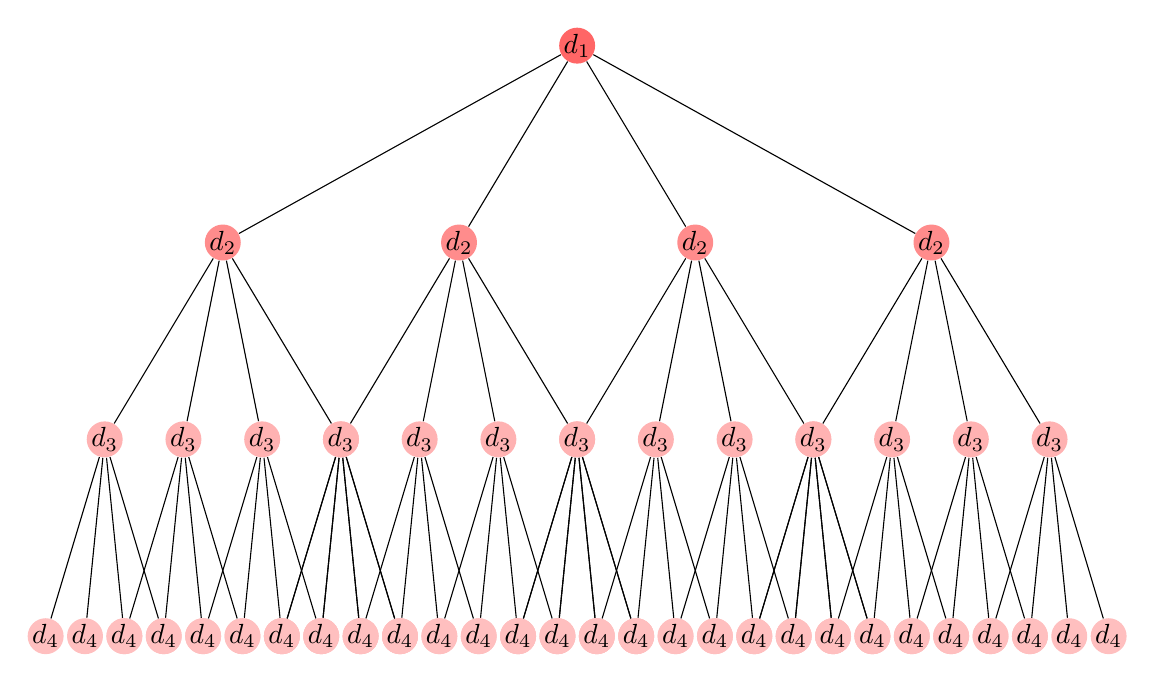
\begin{tikzpicture}
[level distance=25mm,
every node/.style={fill=red!60,circle,inner sep=0.05pt},
level 1/.style={sibling distance=30mm,nodes={fill=red!45}},
level 2/.style={sibling distance=10mm,nodes={fill=red!30}},
level 3/.style={sibling distance=5mm,nodes={fill=red!25}}]

\node  {$d_1$} [grow=down]
child {
	node {$d_2$}
	child {
		node {$d_3$}
		child {
			node {$d_4$}
		}
		child {
			node {$d_4$}
		}
		child {
			node {$d_4$}
		}
		child {
			node {$d_4$}
		}
	}
	child {
		node {$d_3$}
		child {
			node {$d_4$}
		}
		child {
			node {$d_4$}
		}
		child {
			node {$d_4$}
		}
		child {
			node {$d_4$}
		}
	}
		child {
		node {$d_3$}
		child {
			node {$d_4$}
		}
		child {
			node {$d_4$}
		}
		child {
			node {$d_4$}
		}
		child {
			node {$d_4$}
		}
	}
		child {
		node {$d_3$}
		child {
			node {$d_4$}
		}
		child {
			node {$d_4$}
		}
		child {
			node {$d_4$}
		}
		child {
			node {$d_4$}
		}
	}
}child {
	node {$d_2$}
	child {
		node {$d_3$}
		child {
			node {$d_4$}
		}
		child {
			node {$d_4$}
		}
		child {
			node {$d_4$}
		}
		child {
			node {$d_4$}
		}
	}
	child {
		node {$d_3$}
		child {
			node {$d_4$}
		}
		child {
			node {$d_4$}
		}
		child {
			node {$d_4$}
		}
		child {
			node {$d_4$}
		}
	}
		child {
		node {$d_3$}
		child {
			node {$d_4$}
		}
		child {
			node {$d_4$}
		}
		child {
			node {$d_4$}
		}
		child {
			node {$d_4$}
		}
	}
		child {
		node {$d_3$}
		child {
			node {$d_4$}
		}
		child {
			node {$d_4$}
		}
		child {
			node {$d_4$}
		}
		child {
			node {$d_4$}
		}
	}
}
child {
	node {$d_2$}
	child {
		node {$d_3$}
		child {
			node {$d_4$}
		}
		child {
			node {$d_4$}
		}
		child {
			node {$d_4$}
		}
		child {
			node {$d_4$}
		}
	}
	child {
		node {$d_3$}
		child {
			node {$d_4$}
		}
		child {
			node {$d_4$}
		}
		child {
			node {$d_4$}
		}
		child {
			node {$d_4$}
		}
	}
		child {
		node {$d_3$}
		child {
			node {$d_4$}
		}
		child {
			node {$d_4$}
		}
		child {
			node {$d_4$}
		}
		child {
			node {$d_4$}
		}
	}
		child {
		node {$d_3$}
		child {
			node {$d_4$}
		}
		child {
			node {$d_4$}
		}
		child {
			node {$d_4$}
		}
		child {
			node {$d_4$}
		}
	}
}
child {
	node {$d_2$}
	child {
		node {$d_3$}
		child {
			node {$d_4$}
		}
		child {
			node {$d_4$}
		}
		child {
			node {$d_4$}
		}
		child {
			node {$d_4$}
		}
	}
	child {
		node {$d_3$}
		child {
			node {$d_4$}
		}
		child {
			node {$d_4$}
		}
		child {
			node {$d_4$}
		}
		child {
			node {$d_4$}
		}
	}
		child {
		node {$d_3$}
		child {
			node {$d_4$}
		}
		child {
			node {$d_4$}
		}
		child {
			node {$d_4$}
		}
		child {
			node {$d_4$}
		}
	}
		child {
		node {$d_3$}
		child {
			node {$d_4$}
		}
		child {
			node {$d_4$}
		}
		child {
			node {$d_4$}
		}
		child {
			node {$d_4$}
		}
	}
};
\end{tikzpicture}
\end{center}

\noindent Start with a parent node (a digit) say $d_1$. Then, there are $n$ edges (operations) it can travel down to reach the second node (another digit) $d_2$. Then there are once again $n$ edges (operations) it can travel down to reach the third node (some other digit) $d_3$. So on so forth.\\

To find a solution, we traverse every path, accumulating a result along the way. The end result is compared to the goal required to reach.

\pagebreak

\subsection*{Graph Calculations}

\subsubsection*{Single Tree}

\noindent One tree's depth = $m$ digits deep.\\

\noindent At each level of this tree, there are $n$ possible paths to take.\\

\noindent Total paths to traverse $$\sum_{i = 1}^{m} n^{i}$$ in one tree

\subsubsection*{Generalised Trees}

\noindent Generate a tree for every possible permutation of the digits (without repetition), $^{m}P_{m} = m!$ trees to traverse.\\

\subsubsection*{Putting it all together}
Therefore, in a graph approach, we generate a total of

\begin{framed}
$$m! \sum_{i = 1}^{m} n^{i}$$
\end{framed}

statements to evaluated.

\subsubsection*{An Application - Our Example}

Let set of digits to use $D = \lbrace 1, 2, 3, 4 \rbrace$\\
Let set of operations to use $O = \lbrace +, - , \times, \div \rbrace$\\

\noindent $|D| = m = 4$ digits to use\\
$|O| = n = 4$ operations at disposal\\

\noindent Number of brute force statements to evaluate $$m! \sum_{i = 1}^{m} n^{i} = 4!\sum_{i = 1}^{4} 4^{i} = 24 (4 + 4^{2} + 4^{3}) = 2016$$

\end{document}